\section{Hardware}

This section is dedicated to show all the electronic components we chose and how they work together. As described earlier the PCB containing all the components will be manufactured by Seeedstudio. They manufacture PCBs with other hardware components and they sell quite a number of different breakout boards and other developpement parts. A request made by CHIC managing team was to source as many components as possible at Seeedstudio. Of course not all components we needed were available by them so some of the components are from different sources.

We were basically going to build a tablet. It didn't need to have the power of high end tablets of today but it still was quite a challenge. At first we were thinking it would be possible to take an open source ARM chip devellopment board, devellop our application and then take the schematics and rebuild a whole board including the processor, memory, etc.. plus all our peripherals and build the whole device from scratch. But we quickly understood that it was much too complicated to do in a semester. So we decided to take an existing board and build an add-on board hosting our additionnal components.

There are a number of different devellopment/tinkering boards out there. The most famous one might be the raspberry Pi, although quite capable it seemed a little limited for our application (clocked at 700 mhz for the raspberry pi 1). Another problem was that the raspberry pi is not completely open source. Indeed its schematics and gerber files are not available. At the beginning of the project thinking we might build the whole board up from scratch it was necessary for us to work with a totally open source platform which we could build upon.

So we looked into one of the other famous board: the beagle bone black. Which we will further refer to as the BBB. This board clocked at 1 GHz seemed quite capable. There was lots of documentation, a wide community, and especially it is completelly open source hardware and software. This is what we went for.

In fig.\ref{fig:hardware dependencies} we describe the different components of our device and how the connect to each other.

\begin{figure}[!htb]
    \centering
    \includegraphics[width=0.7\textwidth,keepaspectratio]{chap/hardFig/overall_hardware_dependecies}
    \caption{Hardware components dependencies.}
    \label{fig:hardware dependencies}
\end{figure}

\subsection{Beaglebone Black}
The BBB uses an ARM processor from Texas Instruments, the AM335X. It is clocked at 1GHz.

\begin{figure}[!htb]
    \centering
    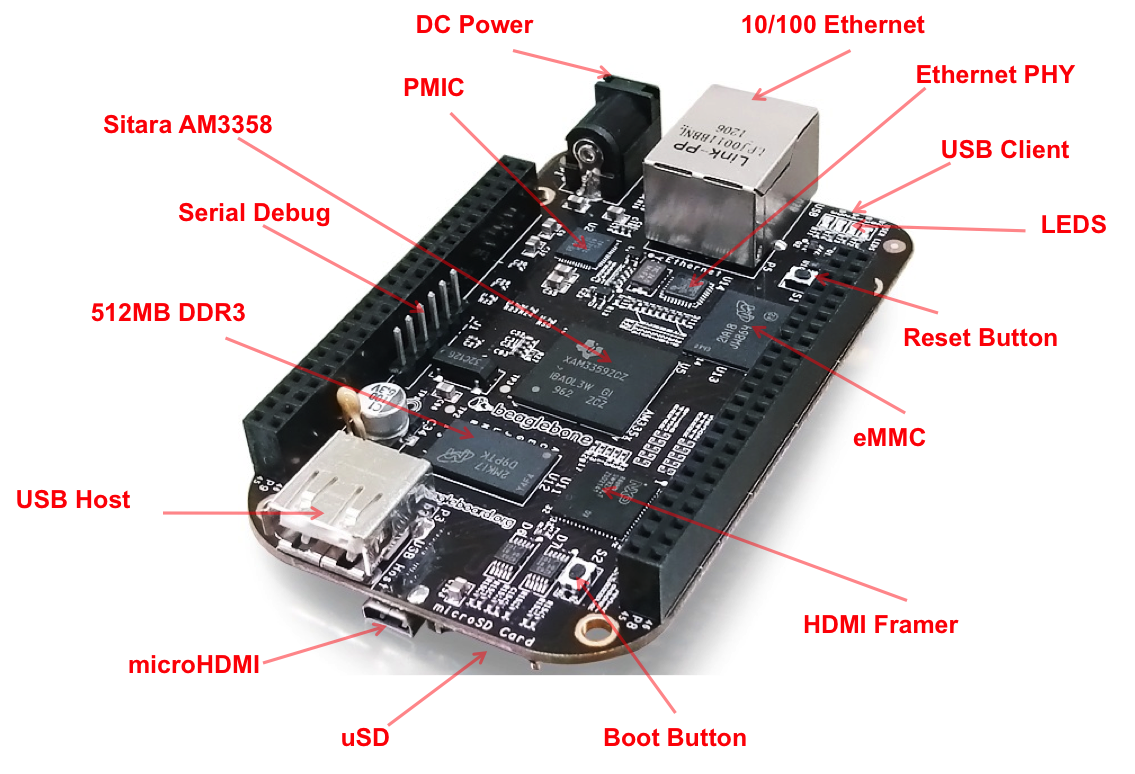
\includegraphics[width=0.7\textwidth,keepaspectratio]{chap/hardFig/bbb.png}
    \caption{Beaglebone black.}
    \label{fig:bbb}
\end{figure}

\begin{itemize}
  \item{ AM335x 1GHz ARM® Cortex-A8 }
  \item{512MB DDR3 RAM}
  \item{4GB 8-bit eMMC on-board flash storage}
  \item{Ethernet}
  \item{2x 46 pin headers}
  \item{Open source}
  \item{...}
\end{itemize}
The main interface of the BBB are the 92 pins. Many pins can be configured in different modes. The pins and modes are listed in fig.\ref{fig:pin modes}.
\clearpage


%\begin{figure}[!htb]
\begin{sidewaysfigure}[h]
    \centering
    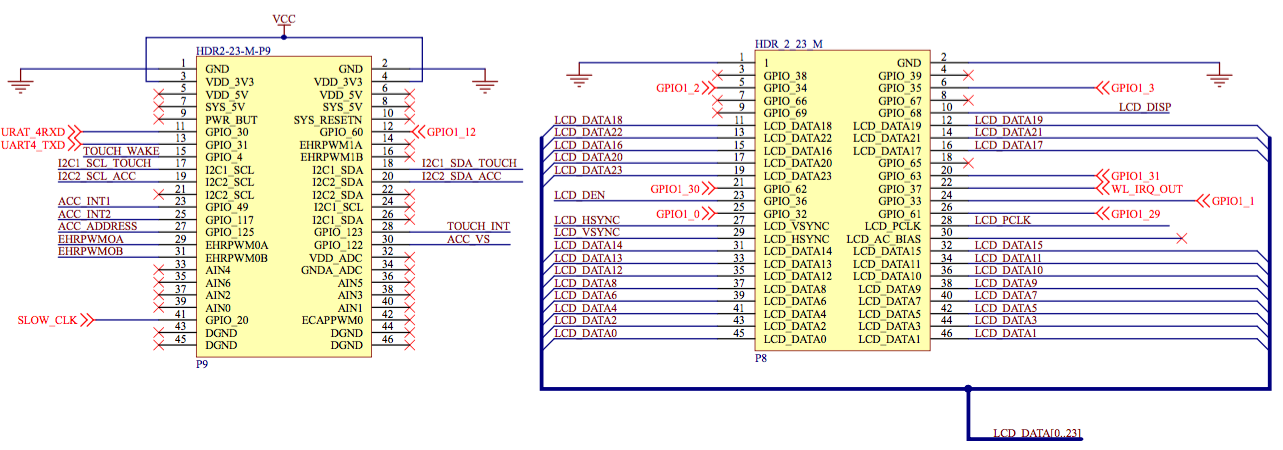
\includegraphics[width=0.9\textwidth,keepaspectratio]{chap/hardFig/BBB_pins_sch}
    \caption{Hardware components dependencies.}
    \label{fig:pin modes}
%\end{figure}
\end{sidewaysfigure}

\clearpage

% \begin{table}[!htbp]
%   \begin{center}
%     \begin{tabular}{|l|r|r|}%p{5cm}|}
%       \hline
%         measurement N$^{\circ}$ & CW [mNm] & CCW [mNm]\\ \hline %\hline
%         test two & 2.24e-4 & -6.32e-4 \\ \hline
%         2 & 2.073-4 & -6.39e-4\\ \hline
%         3 & 2.72e-4 & -6.64e-4\\ \hline
%         4 & 2.46e-4 & -6.46e-4\\ \hline
%         5 & 2.72e.4 & -6.64e-4\\ \hline \hline
%         mean & 2.44e-4 & -6.49e-4\\
%          \hline
%     \end{tabular}
%   \end{center}
%   \caption {Main BBB specifications} \label{tab:bbb specs}
% \end{table}

\subsection{Screen and Touchscreen}
At the current state of our prototype the main function is to view images and text. Therefore a good screen with realistic colors is necessary to have a good user experience.
We first ordered a resistive touchscreen BBB cape (4DCAPE-70T by 4D systems) available from Seeedstudio to see how its was made and to see if the resistive technology was applicable to our project. We quickly realised that the resistive touchscreen was not very suitable to manipulate photos. Especially the very well known “swipe” geasture to move from one photo to another was impossible to do with the resistive touchscreen.
This screens colors were coded on 16 bits and the viewing angle was quite bad. We decided to use a capacitive touchscreen and more colors if possible. We chose a screen we found on Mouser which had good documentation and especially there was an existing driver for the touchscreen IC in the linux kernel we were going to use.
 The screen is actually a package containing the screen and its driver, the touch-screen and its driver and the backlight LED array. This package can be seen in fig.\ref{fig:screen package}

 \begin{figure}[!htb]
     \centering
     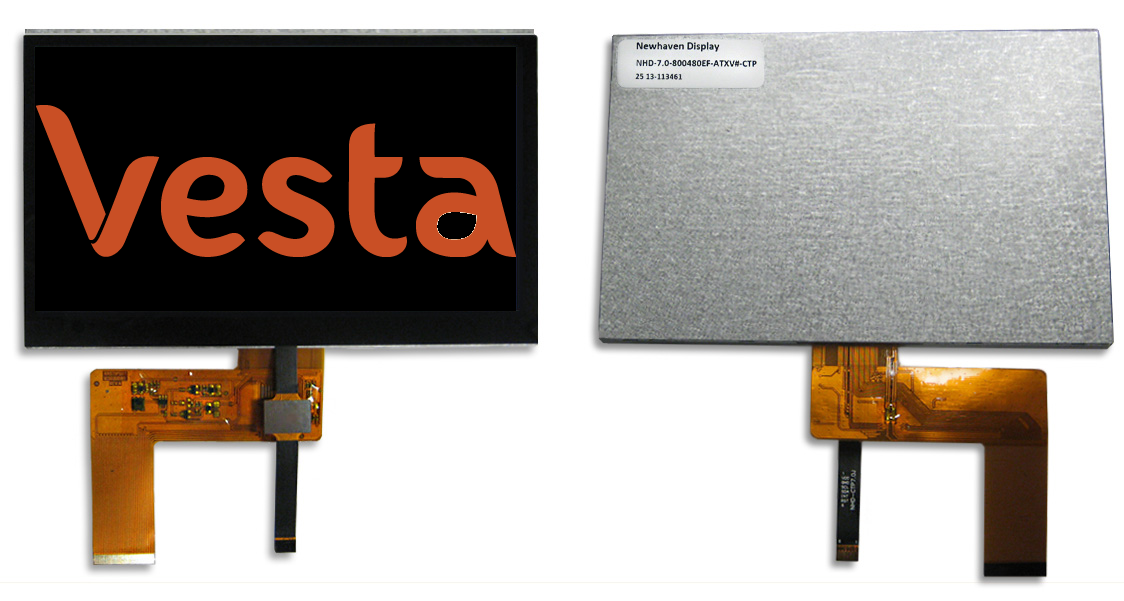
\includegraphics[width=0.5\textwidth,keepaspectratio]{chap/hardFig/newhaven_screen_image}
     \caption{Screen package.}
     \label{fig:screen package}
 \end{figure}

 Individual components are discribed in the following sub chapters.

\subsubsection{Screen}
The screen is the NHD-7.0-800480EF-ATXV\#-CTP from Newhaven Display. The specifications of the screens are listed bellow.
\begin{itemize}
  \item {7" Diagonal}
  \item{Resolution: 800xRGBx480}
  \item{24 bit digital RGB interface}
  \item{White led backlight}
  \item{55-65$^{\circ}$ Top-bottom viewing angle }
  \item{70 $^{\circ}$ left-rigth viewing angle}
\end{itemize}


\subsubsection{Touchscreen}

\begin{itemize}
  \item {Capacitive touch panel with built-in Focaltech ft5x06 controller}
  \item {i2c interface}
  \item {linux kernel compatible}
\end{itemize}
The touchpanel is very smooth and reactive. The
\subsubsection{Backlight}
\label{chap: backlight}
The backlight is a quite bright white led array consisting of 5x3 LEDs. the configuration can be seen in fig.\ref{fig:backlight_led}

\begin{figure}[!htb]
    \centering
    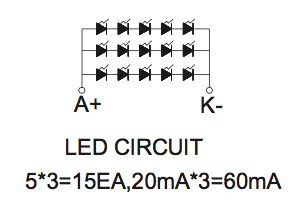
\includegraphics[width=0.5\textwidth,keepaspectratio]{chap/hardFig/backlight_led_circuit}
    \caption{Backlight LED array configuration.}
    \label{fig:backlight_led}
\end{figure}

This LED array requires 60 mA at 16 V to operate. This power is taken directly from the 3.3v of the BBB and boosted to the required voltage by FAN5333A LED driver from Fairchild semiconductors.
This IC is a general purpose LED driver which can be controller with a PWM imput.
Our implementation of the FAN5333B is pictured in fig.\ref{fig:backlight driver schematics}.

\begin{figure}[!htb]
    \centering
    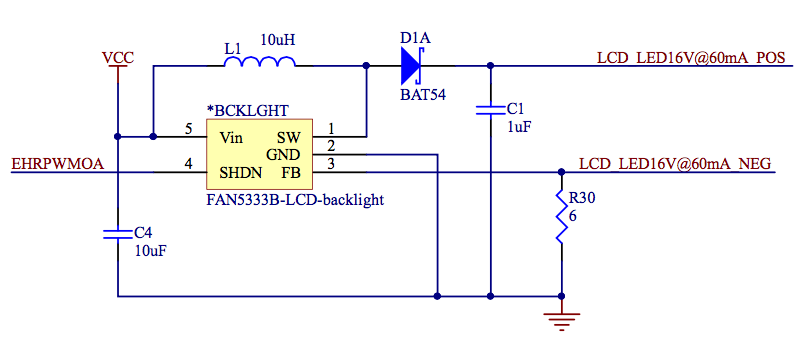
\includegraphics[width=0.7\textwidth,keepaspectratio]{chap/hardFig/backlight_led_driver_sch}
    \caption{FAN5333B Backlight LED driver implementation.}
    \label{fig:backlight driver schematics}
\end{figure}

From the data sheet the resistance R30 regulates the current. The net EHRPWMMOA is connected to a pwm pin on the BBB. The brightness of the screen will be adjustable from the website interface.
\subsection{Wireless Communication}
\label{chap:wireless com}
Our device has to connect to the internet over a WLAN to download new messages from the website. We chose to use the WL1835 chip from Texas instruments. This IC integrates WlAN, 4.1 bluetooth and BLE. An important point is that TI provides support for the linux kernel we are using and the AM335x 1GHz ARM® Cortex-A8.

The chip is provided in a 100-pin MOC package. The pin designation is seen in fig.\ref{fig:wl1835 pin designation}.

\begin{figure}[!htb]
    \centering
    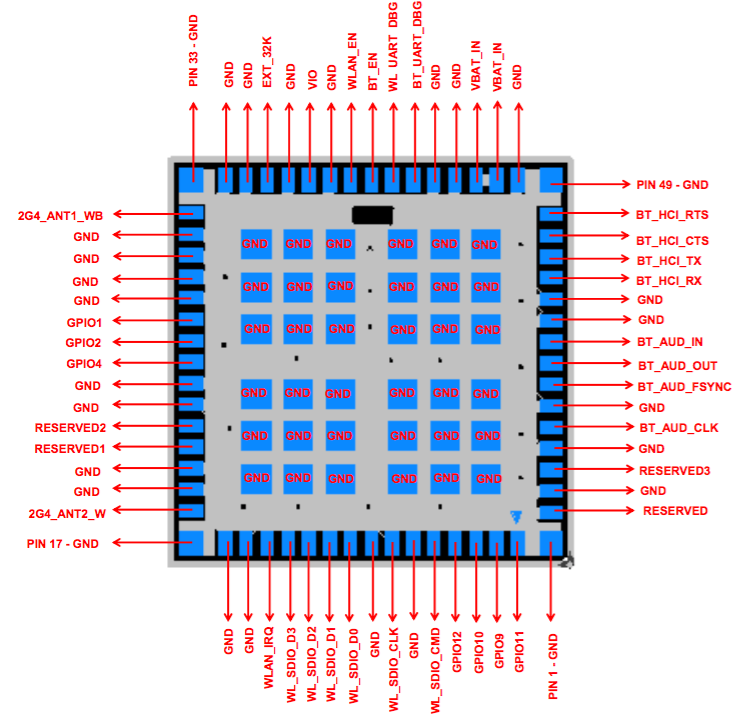
\includegraphics[width=0.5\textwidth,keepaspectratio]{chap/hardFig/100_pin_MOC_wl1835_package}
    \caption{Wl1835 pin designation.}
    \label{fig:wl1835 pin designation}
\end{figure}

To operate the wl1835 needs a few external components. Among others an oscillator and antennas are necessary to for proper operation.
The integration of this chip was inspired by a layout example provided by TI as well as by the layout of an existing BBB cape which can be found here \url{http://boardzoo.com/index.php/beaglebone/beaglebone-wl1835mod-w-chip-antenna.html}.

Our implementation is displayed in fig.\ref{fig:wl1835 chip}



\begin{figure}[!htb]
    \centering
    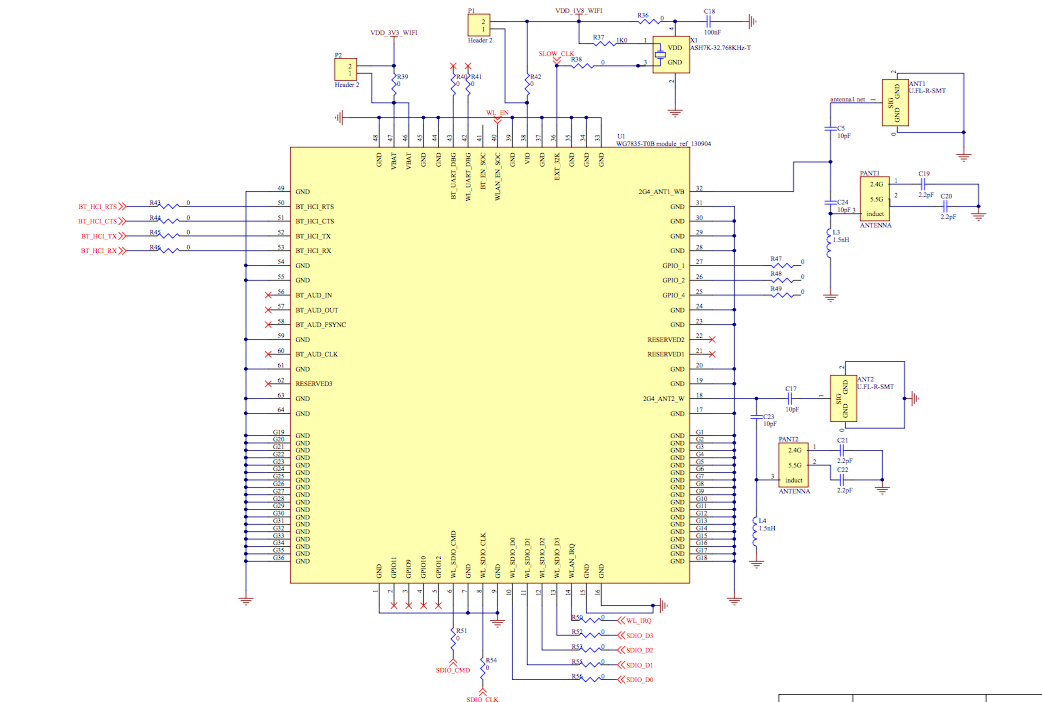
\includegraphics[width=1\textwidth,keepaspectratio]{chap/hardFig/wl1835_chip_sch}
    \caption{Wl1835 implementation.}
    \label{fig:wl1835 chip}
\end{figure}

\subsubsection{Wlan}
The chip supports the IEEE standards 802.11a/b/g/n. This means it can provide up to 100 MPs with UDP and up to 80 MPs with TCP.
It uses a 4 bit SDIO interface to communicate with the BBB. The BBB has 2 SDIO interfaces which are used to communicate with the micro sd card and the onboard EMMC. Therefore using the wl1835 means that we no longer have access to the emmc. This is not a big issue as the operating system can be located on the sd card.


\subsubsection{Bluetooth}
The Wl1835 provides 4.1 bluetooth and low energy bluetooth capabilities. Uart host controlled interface is used to communicate through this interface.

The bluetooth interface is not used currently. It is integrated thinking of future development (see chap.\ref{chap: next steps}).

\subsubsection{Power management}
The WL1835 is quite power hungry, it can pull up to about 500 mA of current and requires both 3.3V and 1.8V to operate. Therefore it has its own linear regulators which pull their current directly from the battery. For the 1.8V the TPS73618DBVR low voltage dropout regulator is used. It can output a maximum of 400 mA at 1.8V more

\begin{figure}[!ht]
    \centering
    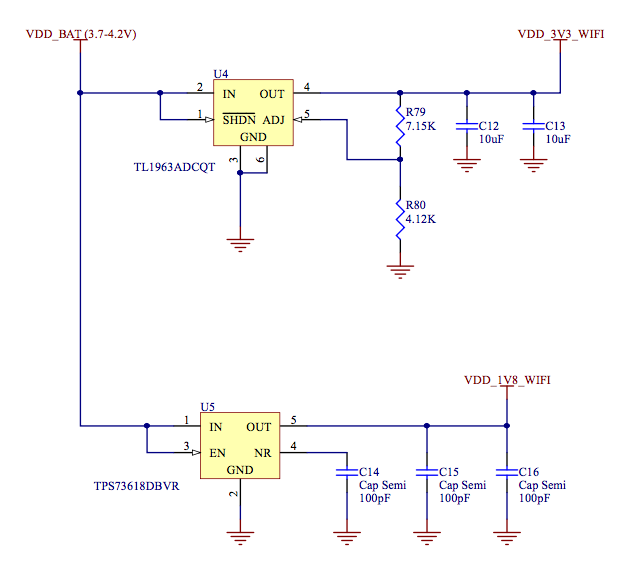
\includegraphics[width=0.7\textwidth,keepaspectratio]{chap/hardFig/wl1835_power_sch}
    \caption{Wl1835 power management implementation.}
    \label{fig:power management}
\end{figure}

\subsubsection{Buffering}
As the signals that come in and out of the wl1835 are 1.6V and the BBB only works with 3.3V, we neeed to used a bidirectional Voltage-Level Translator. We chose the same ones which were implemented in the existing wl1835 cape(see). The TXS0108EPWR from TI.

The implemention of these voltage converters is displayed in fig.\ref{fig:buffering chip}.

\begin{figure}[!ht]
    \centering
    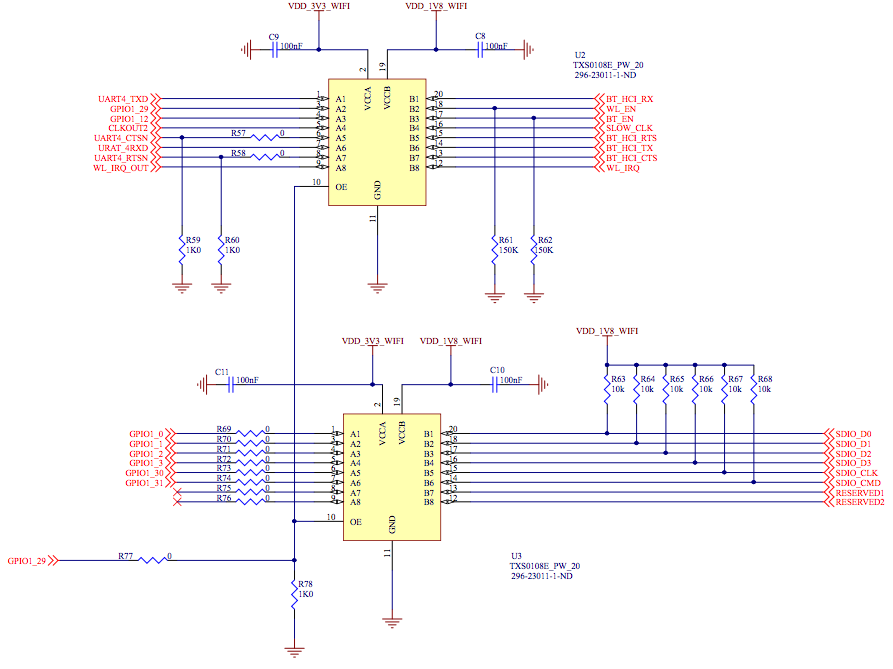
\includegraphics[width=0.7\textwidth,keepaspectratio]{chap/hardFig/wl_1835_buffer_sch}
    \caption{TXS0108EPWR buffering chip implementation.}
    \label{fig:buffering chip}
\end{figure}
\subsubsection{Antennas}
This chip can handle two antennas although only one is compulsory. Again following the TI design guide as well as the schematics of the wl1835 BBB cape mentioned in chap.\ref{chap:wireless com} we implemented a dual antenna design. A ceramic chip was used as the \"on board\" antennas. The layout and custom footprints designed for this part are further described in chap.\ref{chap:pcb}.
\subsection{Front LED}
The LED is there to inform the user of a new message. As it is only a notification LED a 20 mA LED is enough. The same FAN5333B driver for the led array in chap.\ref{chap: backlight} is used. Another PWM pin of the BBB is used to make the LED blink.
\subsection{Power management}
The power source of the device is of course the battery. From the battery the power is channeled into two main groups. The wl1835 wireless chip and the
The two main devices which draw the most current are the BBB and the wifi chip.
The electrical flow is detailed in fig.

\begin{figure}[!ht]
    \centering
    
\includegraphics[width=0.7\textwidth,keepaspectratio]{chap/hardFig/vesta_power_management}
    \caption{Eelctrical flow from the wall outlet to the different components of the device.}
    \label{fig:power flow}
\end{figure}

\subsection{Batteries and charger}
The battery is a 3.7V Lithium-ion battery with a capacity of 6000mAh from Seeedstudio. The voltage of such batteries range from 3.7V to 4.2V. Seeedstudio also sell a li-ion battery charger and wireless power trnasmission coils. We use this system
\subsection{PCB}
\label{chap:pcb}
The PCB was designed in Altium Designer 15. Unfortunatly at this stage no prototype of the PCB has been made. All the components appart from the wl1835 have been tested with the BBB on a breadboard. The complex package of the chip prevents from connecting it to the BBB with wires. The cape mentionned in chap.\ref{chap:wireless com}as source for the wl1835 implementation

\subsubsection{Overall description}
The PCB is composed of four layers. These layers are described in table.\ref{tab:layer description}.
\begin{table}[!htbp]
  \begin{center}
    \begin{tabular}{|l|r|r|r|}%p{5cm}|}
      \hline
        Layer name & type & Material & Thickness [mm] \\ \hline \hline
        Top Overlay & Overlay & & \\ \hline
        Top solder & solder mask & surface material & 0.01 \\ \hline
        Component side & signal & copper &  \\ \hline
        Dielectric 1 & Dielectric & FR-4 & 0.4 \\ \hline
        Ground & GND & copper &\\ \hline
        Dielectric 1 & Dielectric & FR-4 & 0.4 \\ \hline
        Power & VCC & copper & \\ \hline
        Dielectric 1 & Dielectric & FR-4 & 0.4 \\ \hline
        Bottom side & signal & copper &\\ \hline
         \hline
    \end{tabular}
  \end{center}
  \caption {Pcb layer description} \label{tab:layer description}
\end{table}
The power plane is set to the 3.3v of the BBB.

\subsubsection{Antennas}
The chip antennas are the ANT016008LCD2442MA1 from TDK. The datasheet and previously mentioned examples allowed us to design the custom footprint.
The main considerations described by the afrtmentioned sources for the antennas to have maximum efficiency are:

\begin{itemize}
  \item {the antennas are orthogonal to each other}
  \item {They must be distanta of >76 mm which is a half wave length}
  \item {RF traces must have 50-\textOmega impedance}
  \item {RF traces must not have sharp corners}
  \item {RF traces must have via stitching on the ground plane beside the RF trace on both sides}
  \item {RF traces must be as short as possible. The antenna, RF traces, and module must be on the edge of the PCB product in consideration of the product enclosure material and proximity}
\end{itemize}

\begin{figure}[!htb]
    \centering
    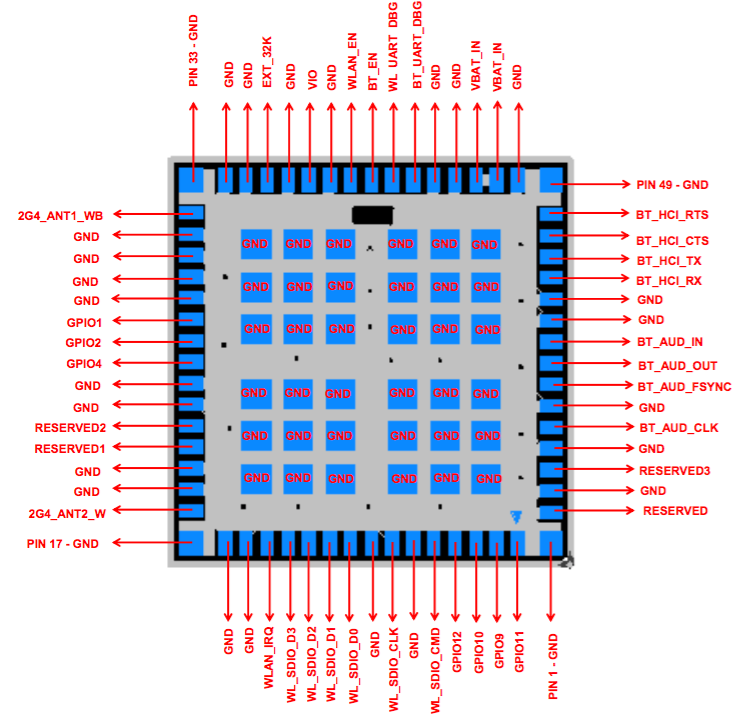
\includegraphics[width=0.5\textwidth,keepaspectratio]{chap/hardFig/100_pin_MOC_wl1835_package}
    \caption{Wl1835 pin designation.}
    \label{fig:wl1835 pcb antennas}
\end{figure}

\subsection{Cost estimates}
